\chapter{The Gauss Code}\label{chap:gauss-code}
\setlength\epigraphwidth{.8\textwidth}
\epigraph{And when he came to the place where the wild things are\\
  they roared their terrible roars and gnashed their terrible teeth\\
  and rolled their terrible eyes and showed their terrible
  claws}{---Maurice Sendak, \emph{Where the Wild Things Are}}

Working with diagrams and Reidemeister moves is significantly better
than working with $3$D objects, but it still has its limitations. What
we really want is a way to represent knots so that we (or, more
likely, a computer) can apply algebraic techniques to this
representation to get us results about knots themselves. This is what
is offered by a combinatorial representation. Essentially, we boil the
information in our diagram down to a finite string in such a way that
we can recover the original diagram losslessly.\footnote{At least, up
  to planar isotopy.} Then, by translating the Reidemeister moves to
permutations on this string, we can view the study of knots in a
purely combinatorial way.

\section{Definitions}
One of the most well-known combinatorial representations is the
\emph{signed Gauss code}:
\begin{definition}[Signed Gauss Code]\label{def:signed-gauss-code}
  Let $K$ be an oriented knot represented as a regular diagram.
  Suppose $K$ has $n$ crossings. Then we encode $K$ in a string
  $コ$\footnote{Katakana \emph{ko}, pronounced \ipa{ko}. Chosen for
    the Katakana transcription of ``code,'' 「コード」。} of
  symbols by the following scheme:
  \begin{enumerate}
    \item Pick some starting point $p_0$ on $K$, and a direction along
      which to transverse $K$.
  \item Starting at $p_0$, begin transversing $K$. Label new crossings
      as with $1, \ldots, n$ in the order that they're encountered.
      Each crossing should be visited exactly twice; we only label a
      crossing the first time.
  \item Whenever we encounter a crossing, we record three pieces of
    information:
    \begin{enumerate}
    \item The crossing label,
    \item whether we're on the under/overstrand, and
    \item the sign of the crossing.
    \end{enumerate}
    We write this compactly by $k_{x}^\epsilon$, where $k \in \set{1,
      \ldots, n}$ is the label we've assigned our crossing, $x \in
      \set{u, o}$ denotes whether we're on the \textbf{u}nderstrand or
      \textbf{o}verstrand, and $\epsilon \in \set{+, -}$ denotes the
      sign of $k$.
  \end{enumerate}
  We call the resulting string of $2n$ characters the \emph{signed
    Gauss code}.\footnote{Note, this definition includes some
    non-standard normalizations, such as labelling the crossings in
    order, and recording the handedness of each crossing \emph{both}
    times it is encountered (instead of just the second). These
    conventions are just to make the correspondence between diagram
    and code clearer, and to give our drawing program a simpler input.
    However, it is completely equivalent to the definition of
    \emph{signed Gauss code} given elsewhere.}
\end{definition}
In the following, it will often be helpful to visualize signed Gauss
codes by \emph{linear diagrams}. Much of the work on the drawing
program\footnote{See
  \href{https://github.com/PythonNut/linear-presentation}{https://github.com/PythonNut/linear-presentation}.
  The project is currently a work-in-progress.} (and on finding
convenient graph encodings) builds on earlier work done jointly with
Jonathan Hayase.
\begin{definition}[Linear Presentation]\label{def:linear-presentation}
  Let $コ$ be a signed Gauss code for an $n$-crossing knot diagram
  $D$. Then a \emph{linear presentation} for $コ$ (also called a
  \emph{linear diagram}) is a knot diagram satisfying the following
  rules:
  \begin{enumerate}
    \item All of the arcs are drawn on grid lines (straight up/down,
      left/right),
    \item All of the crossing points $1, \ldots, n$ are colinear, and
    \item Each crossing $k$ is drawn such that the \np{end of the arc
      corresponding to $k$'s first appearance in the signed Gauss
      code} is horizontal. \qedhere
  \end{enumerate}
\end{definition}
We now record some properties of the signed Gauss code.
\begin{proposition}
  The signed Gauss code has the following properties:
  \begin{enumerate}[label=(\Roman*)]
    \item The substring consisting of \np{the first appearance of each
      crossing in the signed Gauss code} is strictly increasing. E.g.,
      in the \hyperlink{11-2-example}{$(11,2)$} example we have
      {
      \footnotesize
      \[
      1^-_u, 2^-_o, 3^-_o, 4^-_u, 5^+_o, 6^+_u, 7^-_o,
      {\color{lightgray} 3^-_u,}
      8^+_o,
      {\color{lightgray} 5^+_u, 6^+_o,}
      9^+_o, 10^+_u,
      {\color{lightgray} 8^+_u, 4^-_o, 7^-_u,}
      11^-_u,
      {\color{lightgray} 1^-_o, 2^-_u, 10^+_o, 9^+_u, 11^-_o}.
      \]
      }
    \item Two diagrams are \emph{planar} isotopic iff they have the
      same Gauss code (up to the choice of basepoint).\footnote{The
      choice of basepoint corresponds to a cyclic permutation on the
      Gauss code followed by a relabeling.}
    \item Given the signed Gauss code $コ$ for an $n$-crossing knot
      diagram, for all $k = 1,\ldots, n$, there is an even number of
      characters in $コ$ occurring between $k_u$ and $k_o$.
  \end{enumerate}
\end{proposition}
(I) follows immediately from the definition. (II) follows from the
fact that planar isotopies preserve crossings. For (III), a short
proof can be given by noting that the portion of the code between
$k_u$ and $k_o$ (in either direction) defines a closed curve $\gamma$
in the plane. By the Jordan curve theorem, any curve that enters the
region must come back out. This intuition can be used to generate a
short proof.
% \begin{proof}
%   Let $K$ be the underlying knot for the given Gauss code, and let $D$
%   be the diagram. Denote the associated projection by $\pi$. Then
%   $(\pi \circ K) : S^1 \to \RR^2$ is a closed curve.
%   % Suppose, to obtain a contradiction, that there were some $k$ for
%   % which an odd number of characters of $C$ occurred between $k_u$ and
%   % $k_o$. Then there
% \end{proof}

We now provide some examples of signed Gauss codes and associated
linear presentations. Part (3) of
\cref{ex:gauss-codes-and-linear-presentations} might be the most
helpful in understanding part (3) of \cref{def:linear-presentation}.
\begin{example}\label{ex:gauss-codes-and-linear-presentations}~
  \begin{enumerate}
    \item The signed Gauss code $1^+_{u}, 2^{+}_{o}, 3^+_{u},
      1^{+}_o, 2^+_u, 3^+_o$ corresponds to a diagram for the trefoil:
      \begin{figure}[H]
        \centering
        \includegraphics[scale=.55]{figures/background/3_1_0.pdf}
      \end{figure}
    \item The signed Gauss code $1^-_u, 2^-_o, 3^-_u, 4^-_o, 5^-_u,
      6^-_o, 7^-_u, 1^-_o, 6^-_u, 5^-_o, 4^-_u, 3^-_o, 2^-_u, 7^-_o$
      corresponds to a diagram for the $(7,2)$ knot:
      \begin{figure}[H]
        \centering
        \includegraphics[scale=.55]{figures/background/7_2_2.pdf}
      \end{figure}
    \item The signed Gauss code $1^-_u, 2^-_o, 3^-_o,
      4^-_u, 5^+_o, 6^+_u, 7^-_o, 3^-_u, 8^+_o, 5^+_u, 6^+_o, 9^+_o,
      10^+_u, 8^+_u,$ $ 4^-_o, 7^-_u, 11^-_u, 1^-_o, 2^-_u, 10^+_o,
      9^+_u, 11^-_o$ corresponds to the following diagram of the
      \hypertarget{11-2-example}{$(11,2)$} knot:
      \begin{figure}[H]
        \centering
        \includegraphics[scale=.5]{figures/background/11_2_9.pdf}
      \end{figure}
      Note that $8$'s first appearance in the signed Gauss code comes in
      $8^+_o$, hence $8$ is drawn with the overstrand horizontal. This
      is what is meant by part 3 of
      \cref{def:linear-presentation}.\qedhere
  \end{enumerate}
\end{example}
We now examine how the Reidemeister moves can be translated to the
language of the signed Gauss code.

\section{Gauss Codes and Reidemeister
  Moves}\label{sec:gauss-codes-and-reidemeister-moves}
In the context of signed Gauss codes, Reidemeister I corresponds to
insertion/deletion of an adjacent pair:
\begin{figure}[H]
  \centering
  \includegraphics[scale=.5]{figures/background/gauss-moves/gauss-r1.pdf}
  \caption{signed Gauss code Reidemeister I}
\end{figure}
Reidemeister II corresponds to insertion/deletion of a pair of pairs,
albeit with some constraints based on the diagram (see
\hyperlink{note:gauss-code-reidemeister-2}{Note}):
\begin{figure}[H]
  \centering
  \includegraphics[scale=.5]{figures/background/gauss-moves/gauss-r2.pdf}
  \caption{signed Gauss code Reidemeister II}
\end{figure}
Reidemeister III corresponds to swapping three pairs. We have multiple
cases depending on the orientation of the strands; we'll just show two
here:% \footnote{The remaining cases can be obtained by looking at the
% unoriented version of the move with all possible
% orientations/connectivities.}
\begin{figure}[H]
  \centering
  \includegraphics[scale=1.5]{figures/background/gauss-moves/gauss-r3-pair-a.pdf}
\end{figure}
\begin{figure}[H]
  \centering
  \includegraphics[scale=1.5]{figures/background/gauss-moves/gauss-r3-pair-b.pdf}
  \caption{Signed Gauss Code Reidemeister III}
\end{figure}
\begin{note}\label{note:gauss-code-reidemeister-2}
  Given two arcs in a knot diagram, it's not always true that we can
  perform a Reidemeister II move right away. For instance, consider
  the $(5,1)$ knot given by $1_u^+, 2_o^+, 3_u^+, 4_o^+, 5_u^+, 1_o^+,
  2_u^+, 3_o^+, 4_u^+, 5_o^+$:
  \begin{figure}[H]
    \centering
    \includegraphics[scale=.75]{figures/unknotting-moves-and-combinatorial-representations/5_1.pdf}
    \caption{A $(5,1)$ knot}
    \label{fig:Reidemeister-2-planarity-example}
  \end{figure}
  Suppose we wanted to perform a Reidemeister II move crossing the
  $(2^+_u, 3^+_o)$ arc over the $(5^+_o, 1^+_u)$ arc.
  \begin{figure}[H]
    \centering
    \includegraphics[scale=.75]{figures/unknotting-moves-and-combinatorial-representations/5_1_r2_arcs.pdf}
    \caption{A $(5,1)$ Knot.}
    \label{fig:5-1-knot}
  \end{figure}
  If we \emph{only} look at the signed Gauss code rules, this reasonable. We
  just add two new crossings, ${\color{magenta}6},{\color{magenta}7}$
  as follows: $1_u^+, 2_o^+, {\color{magenta} 6_o^{-}}
  {\color{magenta} 7_o^{+}}, 3_u^+, 4_o^+, 5_u^+, 1_o^+, 2_u^+, 3_o^+,
  4_u^+, 5_o^+, {\color{magenta} 7_u^+}, {\color{magenta} 6_u^-}$,
  which would give us something like this in the new diagram:
  \begin{figure}[H]
    \centering
    \includegraphics[scale=.75]{figures/unknotting-moves-and-combinatorial-representations/illegal-r2.pdf}
    \caption{Local View of the Magically-Inserted Crossings}
    \label{fig:magically-inserted-crossings}
  \end{figure}
  However, dutiful examination of \cref{fig:5-1-knot} reveals that
  \cref{fig:magically-inserted-crossings} doesn't make sense. In
  particular, there's no way to add such crossings without first
  introducing \emph{additional} crossings just to get the two strands
  to be adjacent. When we discuss virtual knots later we will do away
  with these petty worldly concerns. For now, however, it is a problem
  we need to address.
\end{note}
To describe things formally, we want to re-interpret the signed Gauss
code (and thus the associated knot diagram) as describing a
combinatorial embedding of a planar graph.\footnote{For those familiar
  with \emph{rotation systems}, the signed Gauss code is really just
  defining one for the kind of 4-valent planar graph shown in
  \cref{fig:crossings-as-vertices}.} Then, we can just say that we're
allowed to do Reidemeister II moves whenever the edges represented by
two arcs are in the same face of the graph.

% \section{The Diagram Graph}
Some care here is required. We can't just treat all of the crossings
as vertices in the new graph and be done with it, because
\hypertarget{planar-point-a}{(a)} this makes it unclear what we mean
when we draw two different identical-looking edges between the same
pair of vertices, and \hypertarget{planar-point-b}{(b)} even then, we
wouldn't be guaranteed a unique planar embedding of the graph, which
would mean we wouldn't have a well-defined notion of ``face'' (see
\cref{fig:crossings-as-vertices}).
\begin{figure}[H]
  \centering
  \includegraphics[scale=.75]{figures/unknotting-moves-and-combinatorial-representations/5-1-planar-graph.pdf}
  \caption[Planar graph]{Naively treating each crossing as a vertex}
  \label{fig:crossings-as-vertices}
\end{figure}
Point \hyperlink{planar-point-a}{(a)} above is referring to the
ambiguity in how we're meant to distinguish between pairs of edges
line like the two from $v_2 \to v_3$ in the figure above. Point
\hyperlink{planar-point-b}{(b)} refers to the fact that even if we
\emph{were} to allow multiple such edges (maybe by labeling the edges
to distinguish them), then both \cref{fig:crossings-as-vertices} and
\cref{fig:alt-crossings-as-vertices} are isomorphic as graphs, but the
faces in each are not the same.
\begin{figure}[H]
  \centering
  \includegraphics[scale=.75]{figures/unknotting-moves-and-combinatorial-representations/5-1-alternative-planar-graph.pdf}
  \caption{A planar graph isomorphic to that in
    \cref{fig:crossings-as-vertices}. Note, the two edges between
    $v_2, v_3$ have been exchanged.}
  \label{fig:alt-crossings-as-vertices}
\end{figure}
There are multiple ways to resolve this problem; the one listed below
is particularly convenient when trying to programmatically reconstruct
diagrams from signed Gauss codes.% \footnote{At this point, it's worth
  % mentioning that other graph encodings \emph{do} exist. One that
  % turns out to be particularly useful in working with bracket-based
  % invariants (e.g., the Kauffman bracket) is \emph{Trace Diagrams}.
  % See \cite{Kobayashi2019Sep}}
Note, the graph below will ``forget''
the sign of the crossings in the knot, but since this turns out to be
very simple to recover from the Gauss code, we ignore it for now.
\begin{definition}[Diagram Graph]\label{def:diagram-graph}
  Given a signed Gauss code $コ$ for an $n$-crossing knot diagram $D$,
  define a planar (undirected) graph representation $G = (V, E)$ of
  the knot as follows:
  \begin{enumerate}[label=(\arabic*)]
    \item \hypertarget{graph-step-1}{} For each $k = 1, \ldots, n$,
      define five vertices $k_u^{\rm in}$, $k_u^{\rm out}$, $k_o^{\rm
      in}$, $k_o^{\rm out}$, and $k^{\rm mid}$. Add them all to $V$.
    \item \hypertarget{graph-step-2}{} For each $k$ as above: add
      edges from $k^{\rm mid}$ to each of $k_u^{\rm in}$, $k_u^{\rm
      out}$, $k_o^{\rm in}$, and $k_o^{\rm out}$ to $E$. Also add the
      edges $\set{k_u^{\rm in}, k_o^{\rm out}}$, $\set{k_o^{\rm out},
      k_u^{\rm out}}$, $\set{k_u^{\rm out}, k_o^{\rm in}}$,
      $\set{k_o^{\rm in}, k_u^{\rm in}}$ to $E$. See
      \cref{fig:local-view-of-a-positive-crossing},
      \cref{fig:local-view-of-a-negative-crossing} for a diagram.
      \begin{figure}[H]
        \centering
        \includegraphics[scale=.75]{figures/unknotting-moves-and-combinatorial-representations/positive-crossing.pdf}
        \caption{Local view of a positive crossing.}
        \label{fig:local-view-of-a-positive-crossing}
      \end{figure}
      \begin{figure}[H]
        \centering
        \includegraphics[scale=.75]{figures/unknotting-moves-and-combinatorial-representations/negative-crossing.pdf}
        \caption{Local view of a negative crossing. Note, the $k_u$'s
          have been swapped relative to
          \cref{fig:local-view-of-a-positive-crossing}.}
        \label{fig:local-view-of-a-negative-crossing}
      \end{figure}
      We have drawn the edges $\set{k_u^{\rm in}, k}$ and $\set{k,
      k_u^{\rm out}}$ dashed to emphasize that they correspond to
      understrands in the knot diagram $D$. The dotted edges are
      dotted to emphasize that they do not appear in the original
      diagram at all.
    \item \hypertarget{graph-step-3}{} For each consecutive pair of
      symbols $\pn{i_{x_i}^{\epsilon_i}, j_{x_j}^{\epsilon_j}}$ in
      $コ$, add the edge $\set{i_{x_i}, j_{x_j}}$ to $E$.
    \item \hypertarget{graph-step-4}{} The steps above are sufficient
      in the case of minimal-crossing diagrams for prime knots (the
      reader might try and verify this after reading the proof of
      \cref{thm:diagram-graph-unique-planar-embedding});
      however, we need to do a bit more for the general case. We'll
      give further exposition on this point \emph{after} we finish
      stating the definition.
      % Motivation for the portion below will be given later in
      % {\color{blue} some figure AAAAAAA}.

      For each $k = 1, \ldots, n$, let $\ell$ be the crossing that comes
      directly after $k$'s first appearance in the signed Gauss code.
      Then define $u_k$, $u_\ell$ and $v_k$, $v_\ell$ such that
      \emph{if} the signed Gauss code were re-indexed to start at $k$,
      then the \emph{right} vertex of $k$ (see
      \cref{fig:local-view-of-a-positive-crossing,fig:local-view-of-a-negative-crossing})
      would be $v_k$, the \emph{top} vertex of $\ell$ would be
      $v_\ell$, the \emph{bottom} vertex of $k$ would be $u_k$, and
      the \emph{left} crossing $\ell$ would be $u_\ell$. Explicitly,
      the casework is as follows.
      % \begin{adjustwidth}{-5em}{-5em}
      \begin{multicols}{2}
        \begin{itemize}
          \item \small $(k^+_u)$: \footnotesize $v_k = k^{\rm out}_u$,
            $u_k = k^{\rm out}_o$
            \begin{itemize}
              \item \small $(\ell_u^+)$: \footnotesize $v_\ell =
                \ell_o^{\rm in}$, $u_\ell = \ell_u^{\rm in}$
              \item \small $(\ell_u^-)$: \footnotesize $v_\ell =
                \ell_o^{\rm out}$, $u_\ell = \ell_u^{\rm in}$
              \item \small $(\ell_o^+)$: \footnotesize $v_\ell =
                \ell_u^{\rm out}$, $u_\ell = \ell_o^{\rm in}$
              \item \small $(\ell_o^-)$: \footnotesize $v_\ell =
                \ell_u^{\rm in}$, $u_\ell = \ell_o^{\rm in}$
            \end{itemize}
          \item \small $(k^-_u)$: \footnotesize $v_k = k^{\rm out}_u$,
            $u_k = k^{\rm in}_o$
            \begin{itemize}
              \item \small $(\ell_u^+)$: \footnotesize $v_\ell =
                \ell_o^{\rm in}$, $u_\ell = \ell_u^{\rm in}$
              \item \small $(\ell_u^-)$: \footnotesize $v_\ell =
                \ell_o^{\rm out}$, $u_\ell = \ell_u^{\rm in}$
              \item \small $(\ell_o^+)$: \footnotesize $v_\ell =
                \ell_u^{\rm out}$, $u_\ell = \ell_o^{\rm in}$
              \item \small $(\ell_o^-)$: \footnotesize $v_\ell =
                \ell_u^{\rm in}$, $u_\ell = \ell_o^{\rm in}$
              % \item \small $(\ell_u^+)$: \footnotesize $u_k = k_o^{\rm in}$, $u_\ell =
              %   \ell_u^{\rm in}$
              % \item \small $(\ell_u^-)$: \footnotesize $u_k = k_o^{\rm in}$, $u_\ell =
              %   \ell_u^{\rm in}$
              % \item \small $(\ell_o^+)$: \footnotesize $u_k = k_o^{\rm in}$, $u_\ell =
              %   \ell_o^{\rm in}$
              % \item \small $(\ell_o^-)$: \footnotesize $u_k = k_o^{\rm in}$, $u_\ell =
              %   \ell_o^{\rm in}$
            \end{itemize}
          \item \small $(k^+_o)$: \footnotesize $v_k = k_o^{\rm out}$,
            $u_k = k_u^{\rm in}$
            \begin{itemize}
              \item \small $(\ell_u^+)$: \footnotesize $v_\ell =
                \ell_o^{\rm in}$, $u_\ell = \ell_u^{\rm in}$
              \item \small $(\ell_u^-)$: \footnotesize $v_\ell =
                \ell_o^{\rm out}$, $u_\ell = \ell_u^{\rm in}$
              \item \small $(\ell_o^+)$: \footnotesize $v_\ell =
                \ell_u^{\rm out}$, $u_\ell = \ell_o^{\rm in}$
              \item \small $(\ell_o^-)$: \footnotesize $v_\ell =
                \ell_u^{\rm in}$, $u_\ell = \ell_o^{\rm in}$
              % \item \small $(\ell_u^+)$: \footnotesize $u_k = k_u^{\rm in}$, $u_\ell =
              %   \ell_u^{\rm in}$
              % \item \small $(\ell_u^-)$: \footnotesize $u_k = k_u^{\rm in}$, $u_\ell =
              %   \ell_u^{\rm in}$
              % \item \small $(\ell_o^+)$: \footnotesize $u_k = k_u^{\rm in}$, $u_\ell =
              %   \ell_o^{\rm in}$
              % \item \small $(\ell_o^-)$: \footnotesize $u_k = k_u^{\rm in}$, $u_\ell =
              %   \ell_o^{\rm in}$
            \end{itemize}
          \item \small $(k^-_o)$: \footnotesize $v_k = k_o^{\rm out}$,
            $u_k = k_u^{\rm out}$
            \begin{itemize}
              \item \small $(\ell_u^+)$: \footnotesize $v_\ell =
                \ell_o^{\rm in}$, $u_\ell = \ell_u^{\rm in}$
              \item \small $(\ell_u^-)$: \footnotesize $v_\ell =
                \ell_o^{\rm out}$, $u_\ell = \ell_u^{\rm in}$
              \item \small $(\ell_o^+)$: \footnotesize $v_\ell =
                \ell_u^{\rm out}$, $u_\ell = \ell_o^{\rm in}$
              \item \small $(\ell_o^-)$: \footnotesize $v_\ell =
                \ell_u^{\rm in}$, $u_\ell = \ell_o^{\rm in}$
              % \item \small $(\ell_u^+)$: \footnotesize $u_k = k_u^{\rm out}$, $u_\ell =
              %   \ell_u^{\rm in}$
              % \item \small $(\ell_u^-)$: \footnotesize $u_k = k_u^{\rm out}$, $u_\ell =
              %   \ell_u^{\rm in}$
              % \item \small $(\ell_o^+)$: \footnotesize $u_k = k_u^{\rm out}$, $u_\ell =
              %   \ell_o^{\rm in}$
              % \item \small $(\ell_o^-)$: \footnotesize $u_k = k_u^{\rm out}$, $u_\ell =
              %   \ell_o^{\rm in}$
            \end{itemize}
        \end{itemize}
      \end{multicols}
      % \end{adjustwidth}
      % From the signed Gauss code, one can compute what the ``bottom''
      % and ``right'' vertices for $k$ defined in
      % % crossings $k$ and $k + 1$
      % % (for $k = n$, take crossing $1$ instead of
      % % $k+1$).\footnote{Choosing to index starting at $1$ instead of
      % % indexing at $0$ has causes a bit of a headache in explicitly
      % % describing the labeling in the case of $k = n$. We hope the
      % % meaning is clear in the below --- if not, it can be remedied by
      % % relabeling all the crossings with $0, \ldots, n-1$, and making
      % % the replacement $(k, k+1) \mapsto (k-1, k \mod n)$.} Define
      % % $v_k$, $u_{k}$, $v_{k+1}, u_{k+1}$ to be chosen from the
      % % existing vertices as follows:
      % \begin{itemize}
      %   \item
        % \item To select $u_k, v_k$: If the first occurrence of
        %   crossing $k$ in $C$ corresponds to an undercrossing, then
        %   let $v_k = k_u^{\rm out}$ and
        %   \begin{itemize}
        %     \item if $k$ is positive, let $u_k = k_o^{\rm out}$.
        %     \item if $k$ is negative, let $u_k = k_o^{\rm in}$.
        %   \end{itemize}
        %   If, on the other hand, it is an overcrossing, let $v_k =
        %   k_o^{\rm out}$ and
        %   \begin{itemize}
        %     \item if $k$ is positive, let $u_k = k_u^{\rm in}$.
        %     \item if $k$ is negative, let $u_k = k_u^{\rm out}$.
        %   \end{itemize}
        % \item To select $u_{k+1}, v_{k+1}$ (resp.\ $u_1, v_1$ when $k
        %   = n$): If the first occurrence of crossing $k+1$ is an
        %   undercrossing, then
        %   \begin{itemize}
        %     \item If $k+1$ is positive, let $u_k = \np{k+1}_o^{\rm in}$.
        %     \item If $k+1$ is negative, let $u_k = \np{k+1}_o^{\rm out}$.
        %   \end{itemize}
        %   If, on the other hand, it is an overcrossing, then
        %   \begin{itemize}
        %     \item If $k+1$ is positive, let $u_k = \np{k+1}_u^{\rm out}$.
        %     \item If $k+1$ is negative, let $u_k = \np{k+1}_u^{\rm in}$.
        %   \end{itemize}
      % \end{itemize}
      Finally, add the edges $\set{u_k, u_{\ell}}$, $\set{v_k,
      v_{\ell}}$ to $E$.
  \end{enumerate}
  Then we define the resulting $G = (V, E)$ to be the \emph{diagram
    graph}.\qedhere
\end{definition}
See \cref{fig:ex-knot-graph} on page \cpageref{fig:ex-knot-graph} for
an example of the full diagram graph for the $(5,1)$ knot. Note, part
\hyperlink{graph-step-4}{(4)} of \cref{def:diagram-graph} is meant to
address situations like the following: Consider the segment contained
in the dashed region of \cref{fig:ex-knot-graph}.\footnote{For
  reference, the signed Gauss code for this diagram is given by
  $1_u^+, 2_o^+, 3_u^+, 4_u^+, 5_o^+$, $ 6_u^+, 4_o^+, 5_u^+, 6_o^+,
  1_o^+, 2_u^+, 3_o^+$.}
% \begin{sidewaysfigure}[H]
\begin{landscape}
  \begin{figure}[H]
    \centering
    \includegraphics[scale=.9]{figures/unknotting-moves-and-combinatorial-representations/5-1-knot-graph.pdf}
    \caption[$(5,1)$ diagram graph]{Example of the diagram graph for
      the diagram of $(5,1)$ shown in \cref{fig:5-1-knot}. The dashed
      edges are the ones added in in step
      \hyperlink{graph-step-4}{(4)} of \cref{def:diagram-graph}. See
      below for more.}
    \label{fig:ex-knot-graph}
  \end{figure}
\end{landscape}
% \end{sidewaysfigure}
\begin{figure}[H]
  \centering
  \includegraphics[scale=.7]{figures/unknotting-moves-and-combinatorial-representations/3-1-csum-boxed.pdf}
  \caption{An example knot.}
  \label{fig:graph-def-motivation}
\end{figure}
Suppose we were to omit the edges from step
\hyperlink{graph-step-4}{(4)} of \cref{def:diagram-graph}. Then
observe that, holding the rest of the graph constant, mirroring the
region yields a valid graph isomorphism (\cref{fig:undesirable-flip}).
\begin{figure}[H]
  \centering
  \begin{minipage}{.8\textwidth}
    \begin{turn}{90}
      \centering
      \includegraphics[scale=.6125]{figures/unknotting-moves-and-combinatorial-representations/3-1-knot-and-flip.pdf}
    \end{turn}
  \end{minipage}
  \caption{A valid graph isomorphism.}
  \label{fig:undesirable-flip}
\end{figure}
However, this would change our graph from representing the knot in
\cref{fig:graph-def-motivation} to representing the following:
\begin{figure}[H]
  \centering
  \includegraphics[scale=.7]{figures/unknotting-moves-and-combinatorial-representations/3-1-csum-2.pdf}
\end{figure}
As the two are not even ambient isotopic, this is undesirable.
Thankfully, part \hyperlink{graph-step-4}{(4)} of
\cref{def:diagram-graph} prevents this by adding auxiliary edges as
follows. Consider the following neighborhood of the original knot:
\begin{figure}[H]
  \centering
  \includegraphics[scale=.7]{figures/unknotting-moves-and-combinatorial-representations/3-1-csum-boxed-2.pdf}
  \caption{A neighborhood of crossings $3$ and $4$}
  \label{fig:new-neighborhood}
\end{figure}
In the knot graph \emph{with} the edges added by part
\hyperlink{graph-step-4}{(4)}, the neighborhood appears as follows:
\begin{figure}[H]
  \centering
  \includegraphics[]{figures/unknotting-moves-and-combinatorial-representations/3-1-c3-c4-zoom.pdf}
  \caption{Zoomed view of the neighborhood of
    \cref{fig:new-neighborhood} in the diagram graph}
\end{figure}
We now show that the diagram graph has a unique planar embedding. To
that end, we'll make heavy use of the following theorem of
Whitney.\footnote{For a nice treatment of this theorem, see
  \cite{Bondy2008}. The theorem itself is stated as {\scshape Theorem
    10.28} on pg.\ 267.}
\begin{theorem}[Whitney]\label{thm:whitney}
  Let $G$ be a simple graph planar graph. Suppose $G$ is
  $3$-connected. Then $G$ has a unique\footnote{Here, ``unique'' means
    that any other embedding of $G$ has the same set of faces
    (considered as sets of edges).} planar embedding.
\end{theorem}
There are three hypotheses we need to verify: $G$ is simple, $G$ is
planar, and $G$ is 3-connected.\footnote{Recall, a graph is called
  \emph{$k$-connected} if it has more than $k$ vertices, and removing
} Simplicity follows by construction. Planarity and $3$-connectedness
are slightly more involved, so we'll treat them separately in the
below. In both cases, the following vocabulary will be helpful.
\begin{definition}[Crossing subgraph, underlying crossing, and
  representing vertices]
  Let $コ$ be a signed Gauss code for a regular diagram $D$, and let $G
  = (V,E)$ be the associated diagram graph. Let $v = k_x^{\square} \in
  V$, where $x \in \set{u,o,\ph}$ and $\square \in \set{{\rm in, mid,
      out}}$.\footnote{Note, $x$ is the blank character only when we
    have $k^{\rm mid}$} Let $G_k$ be given by $V_k = \set{k^{\rm
      mid}, k_u^{\rm in}, k_u^{\rm out}, k_o^{\rm in}, k_o^{\rm out}}$
  and all their edges.\footnote{Explicitly, $E_k = \set{\set{v_1,
        v_2} \in E \MID v_1, v_2 \in V'}$.} Then we call
  \begin{itemize}
    \item $G_k$ the \emph{crossing $k$ subgraph} of $G$,
    \item $k$ the \emph{underlying crossing} of $v$, and
    \item $V_k$ the set of \emph{representing vertices} of $k$.
      \qedhere
  \end{itemize}
\end{definition}
Ok --- first, we show the diagram graph is planar.
\subsection{The Diagram Graph is Planar}
Recall, a \emph{subdivision} of a graph $G = (V, E)$ is obtained by
inserting vertices into the middle of edges of
$E$.\footnote{Explicitly: let $e = \set{v_1, v_2} \in E$. Then (a)
  define a new vertex $v'$ and add it to $V$, (b) delete the edge
  $\set{v_1, v_2}$ from $E$, and (c) add $\set{v_1, v'}$, $\set{v',
    v_2}$ to $E$.} The following is a well-known result.\footnote{See
  {\scshape Proposition 10.3} on pg.\ 246 of \cite{Bondy2008}.}
\begin{proposition}\label{prop:subdivision-planarity}
  Let $G = (V,E)$ be an arbitrary graph. Then $G$ is planar iff every
  subdivision of $G$ is planar.
\end{proposition}
The following proposition is also straightforward to prove. We will
actually only need the special case where we are connecting $v_0$ and
$v_2$ (where $v_0, v_1, v_2$ are consecutive vertices in a face), but
the proof is completely identical, so we kept the more general
version.
\begin{proposition}\label{prop:adding-edges-in-face}
  Let $G = (V, E)$ be a planar graph. Consider an arbitrary planar
  embedding of $G$ (denote it $\ms E$), and let $v_0, v_1$ be two
  vertices on some face $F$ of $\ms E(G)$. Then $G' = (V, E \cup
  \set{\set{v_0, v_1}})$ is planar.
\end{proposition}
\begin{sproof}[Sketch]
  We proceed by construction. By definition of a face, $F$ is a
  connected subset of $\RR^2$ such that $F \cap \ms E(G) =
  \varnothing$ and $\partial \ol{F} \subseteq \ms E(G)$.

  Observe that closure preserves connectedness, hence $\ol{F}$ is
  connected. Since we're working in $\RR^2$, connected implies path
  connected, so $\ol{F}$ is path connected. Thus there exists a path
  $\gamma : [0,1] \into F$ with $\gamma(0) = \ms E(v_0)$ and
  $\gamma(1) = \ms E(v_1)$. We define use this to define the embedding
  of $G'$ by\footnote{Recall that we use $\fim{f}{A}$ to denote ``the
    image of $A$ under $f$.''}
  \[
    \ms E'(\square) =
    \begin{cases}
      \ms E(\square) & \text{if } \square \in V \text{ or } \square \in E, \\
      \fim{\gamma}{[0,1]} &\text{if } \square = \set{v_0, v_1}
    \end{cases}
  \]
  Since $F \cap \ms E(G) = \varnothing$, it follows that
  $\fim{\gamma}{[0,1]} \cap \ms E(G) = \varnothing$. Hence the new
  edge doesn't cross any of the embeddings of the previous edges. Thus
  $\ms E'$ is a planar embedding too.
\end{sproof}
Now we can show that the diagram graph is planar.
\begin{proposition}[Planarity of Diagram Graph]
  Let $コ$ be the signed Gauss code for an $n$-crossing knot diagram
  $D$, and let $G = (V, E)$ be the associated diagram graph. Then $G$
  is planar.
\end{proposition}
\begin{sproof}
  Note that by definition of a regular diagram, the non-simple graph
  $G_0 = (V_0, E_0)$ defined by
  \begin{enumerate}
    \item $V_0$ is the set of crossing points of $D$ (labeled
      $1,\ldots, n$), and
    \item $E_0 = \set{\set{u_0,v_0} \in V_0 \MID u_0, v_0 \text{ are
      the endpoints of a semiarc of } D}$
  \end{enumerate}
  is planar (see \cref{fig:crossings-as-vertices}).\footnote{Sketch:
    The knot diagram trivially gives an embedding of the graph, since
    by definition crossings only occur at points of $V_0$, so we can
    just take the semi-arcs to be embeddings of the edges, and all the
    boxes get ticked.} Observe that taking $k^{\rm mid} = k$ and then
  performing step \hyperlink{graph-step-1}{(1)}, the first part of
  step \hyperlink{graph-step-2}{(2)}, and step
  \hyperlink{graph-step-3}{(3)} of \cref{def:diagram-graph}
  corresponds to taking a subdivision of $G_0$.\footnote{These steps
    were: \np{step \hyperlink{graph-step-1}{(1)}} adding the
    representative vertices, \np{first part of
      \hyperlink{graph-step-2}{(2)}} adding all the spokes from
    $k^{\rm mid}$ to the other representative vertices, and \np{step
      \hyperlink{graph-step-3}{(3)}} connecting the rims of the
    crossing $k$ subgraphs together as dictated by the signed Gauss
    code.} In particular, we have subdivided each edge $\set{v_i,
    v_j}$ twice by inserting an ``out'' vertex and an ``in'' vertex,
  assigned to $v_i, v_j$ as dictated by the signed Gauss code. Thus,
  by \cref{prop:subdivision-planarity}, the resulting graph $G_1 =
  (V_1, E_1)$ is planar.

  Now observe that by \cref{prop:adding-edges-in-face}, performing the
  second part of step \hyperlink{graph-step-2}{(2)} (adding the rims
  to each of the crossing $k$ subgraphs) yields a new planar graph
  $G_2$.\footnote{If being extremely rigorous, one would need to argue
    that none of these added edges can ever cross \emph{each other}.
    This is straightforward: the crossing $k$ subgraphs are each
    planar (since they're isomorphic to $W_4$), and we haven't added
    edges anywhere else.} A similar argument can be applied to show
  that step \hyperlink{graph-step-4}{(4)} corresponds to applying
  \cref{prop:adding-edges-in-face} to $G_2$, hence the resulting graph
  $G_3$ is planar as well. Since $G_3$ is the diagram graph itself, we
  now have the desired result.
\end{sproof}
Now, we show the diagram graph is $3$-connected.
\subsection{The Diagram Graph is 3-Connected}
We start by proving that each crossing $k$ subgraph is $3$-connected,
then we use this to argue the case for the diagram graph.
\begin{lemma}\label{lem:crossing-k-subgraph-3-connected}
  Let $コ$ be a signed Gauss code for a regular $n$-crossing diagram
  $D$, and let $G = (V,E)$ be the associated diagram graph. Then for
  all $k = 1, \ldots, n$, the crossing $k$ subgraph is $3$-connected.
\end{lemma}
\begin{sproof}
  Note that for all $k$, by construction, $G_k$ is isomorphic to the
  wheel graph $W_4$. One can do a brute-force check to verify $W_4$ is
  $3$-connected\footnote{A straightforward way is to apply Menger's
    theorem and argue that between any two vertices, there exist $3$
    internally vertex-disjoint paths (fancy way of saying paths that
    are disjoint except the endpoints). One can use the symmetry of
    $W_4$ to reduce the argument to just $3$ cases: (1) two adjacent
    vertices on the rim, (2) two opposite vertices on the rim, and (3)
    the center vertex with any other vertex.}
\end{sproof}
Now, we attack the diagram graph.%  We prove a weaker result first.
% \begin{lemma}
%   Let $C$ be a signed Gauss code for a regular $n$-crossing diagram
%   $D$, and let $G = (V,E)$ be the associated diagram graph. Then $G$
%   is at least $2$-connected.
% \end{lemma}
% \begin{sproof}[Sketch]
%   Let $v_0, v_1 \in V$ with $v_0 \neq v_1$ be arbitrarily chosen. We
%   want to show there are at least two disjoint paths from We
%   have two sub-cases.
%   \begin{enumerate}
%     \item Suppose $v_0$, $v_1$ have the same underlying crossing. Then
%       by \cref{lem:crossing-k-subgraph-3-connected},
%   \end{enumerate}
% \end{sproof}
% We have the following corollary, the proof of which is quite
% straightforward.
% \begin{corollary}
%   Let $G = (V,E)$ be quantified as above. Then for all $v \in V$,
%   $\deg(v) \geq 3$, with equality holding iff the underlying crossing
%   of $v$ can be removed with a Reidemeister I move.
% \end{corollary}
% \begin{sproof}
%   Let $k$ be the underlying crossing of $v$. Note, $\deg(v) \geq 3$
%   follows from the fact that $G_k$ is a wheel graph. It remains to
%   show that $\deg(v) = 3$ iff $k$ can be removed with a Reidemeister I
%   move.
%   \begin{iffproof}
%     \item Suppose that $\deg(v) = 3$. By construction, this can only
%       occur when the next character in the signed gauss code is
%     \item
%   \end{iffproof}
% \end{sproof}

\begin{theorem}\label{thm:diagram-graph-unique-planar-embedding}
  Given a signed gauss code $コ$ for an $n$-crossing knot diagram $D$,
  there exists a unique planar embedding of the associated diagram
  graph $G = (V, E)$.
\end{theorem}
\begin{proof}
  Again, by \cref{thm:whitney}, we want to show that $G$ is
  $3$-connected. To that end, consider an arbitrary cut $(S,T)$ of
  $G$, and let the cut-set be $E_{\rm cut}$.\footnote{Recall, a cut is
    a partition of $V$ into two disjoint sets $S$, $T \neq
    \varnothing$, such that the subgraphs $G_S = (S, E\mid_S)$, $G_T =
    (T, E\mid_T)$ (where $E\mid_S$, $E\mid_T$ denote is the original
    edge set restricted to $S$, $T$ respectively) are connected. The
    set of edges bridging $G_S, G_T$ in $G$ is defined to be the
    \emph{cut-set}, denoted $E_{\rm cut} = \set{\set{s,t} \in E \MID s
      \in S, t \in T}.$} We want to show $\abs{E_{\rm cut}} \geq 3$.
  We have two subcases.

  \begin{enumerate}
    \item Suppose $E_{\rm cut}$ contains an edge from one of the
      crossing $k$ subgraphs, denote it $G_k$. Then $S,T$ partition
      $G_k$, and by \cref{lem:crossing-k-subgraph-3-connected}, we
      have at least $3$ edges in $E_{\rm cut}$, as desired.
    \item  Now suppose $E_{\rm cut}$ does not contain an edge from any
      of the crossing $k$ subgraphs. Then $S, T$ partition the
      crossing $k$ subgraphs. By the pigeonhole principle, there
      exists some $k$ such that if $\ell$ is the crossing that comes
      directly after $k$'s first appearance in the signed Gauss code,
      the representing vertices $V_k$, $V_\ell$ satisfy $V_k
      \subseteq S$, and $V_\ell \subseteq T$.\footnote{To argue this:
      first note that the case where there's only $1$ crossing
      subgraph is covered by the first case. Hence, without loss of
      generality $n \geq 2$. Now observe that there are $n$ such $k,
      \ell$ pairs, and only two sets to partition them across.}

      Recall the definitions of $u_k$, $u_\ell$, $v_k$, $v_\ell$ from
      \cref{def:diagram-graph} step \hyperlink{graph-step-4}{(4)}.
      Note that $u_k$, $u_\ell$ and $v_k$, $v_\ell$ are distinct. Thus
      the edges $\set{u_k, u_\ell}$, $\set{v_k, v_\ell}$, $\set{v_k,
      u_\ell}$ are all distinct. The first two are added in step
      \hyperlink{graph-step-4}{(4)}, the latter in step
      \hyperlink{graph-step-3}{(3)}. Thus $\abs{E_{\rm cut}} \geq 3$,
      as desired.
  \end{enumerate}
  Since these cases are exhaustive, we have $\abs{E_{\rm cut}} \geq
  3$, as desired.
\end{proof}
Huzzah! Now, we can \emph{finally} go back and clear up the problems
with the Gauss code Reidemeister II move. In particular, we have
\begin{proposition}
  We can perform a Reidemeister II move on two semi-arcs of a
  regular diagram $D$ iff they are part of a shared face in the
  diagram graph $G$.
\end{proposition}
The proof follows directly from the construction.
% \begin{sproof}[Sketch]
  % Follows from construction. Given any embedding of $G$, we can take
  % an ambient isotopy similar to

 % {\color{blue} that one on the triangle
  % thingies later AAAAAAAAAaa}
% \end{sproof}

\subsection{Some More Notes on the Diagram Graph}
With the (admittedly significant) planarity constraints on the diagram
graph, we can encode our knots losslessly up to a choice of chiraliy,
as described in the following proposition.
\begin{proposition}
  For knots $K_0$, $K_1$ with diagrams $D_0$, $D_1$, the associated
  diagram graphs $G_0$, $G_1$ are isomorphic iff $D_0$ and $D_1$ are
  equivalent by planar isotopy together with (at most) a single
  reflection.
  % For a knot $K$ with diagram $D$, $K$ and its mirror image have
  % isomorphic diagram graphs.
\end{proposition}
Again, this follows more or less by construction. The upshot is that
we can now fully encode knot equivalence by moves on the signed Gauss
code subject to planarity constraints.\footnote{Alternatively, we can
  encode the Gauss code Reidemeister moves directly in moves on the
  diagram graph.}

\begin{proposition}
  Given: two sets $V, E$ representing a diagram graph $G$, there
  exists a greedy algorithm for enumerating the faces of the $G$ that
  runs in $O(n)$ time (where $n = \abs{V}$).
\end{proposition}
\begin{sproof}
  % Note that the vertices in the graph have bounded degree, hence the
  % total number of edges is $O(n)$. The exact

  Initialize an empty list of faces. Subdivide each edge in the graph
  into two directed half-edges with opposite orientations ($O(n)$).
  Note of these, there are only $4n$ edges that we're actually
  interested in (the half-edges representing arcs in the diagram).
  Also observe that each half-edge is contained in exactly 1 face of
  $G$.

  Initialize a counter to $0$ to keep track of how many half edges
  we've seen so we know when to stop. Choose an arbitrary starting
  edge, and perform an $O(1)$ check to make sure it's not the interior
  half-edge for one of the vertex-$k$ subgraphs. If it is, then it's
  another $O(1)$ operation to find a correct starting point (this can
  be done by adding casework to navigate through the vertex
  $k$-subgraph).

  Once at a valid starting point, follow the graph counterclockwise
  around the boundary of each face, popping half-edges off as they are
  encountered. Observe that throughout this process, the decision of
  ``which edge to traverse next'' can always be made in $O(1)$ time
  because the rim vertices of the vertex $k$ subgraphs are canonically
  ordered.\footnote{In terms of implementation, we can do something
    simple like representing each vertex by a tuple $(v,
    \text{label})$ where label encodes the under/over/in/out/mid
    information, or by representing the vertices as integers where
    $k^{\rm mid} \mapsto 5k$, $k^{\rm out}_u \mapsto 5k+1$, etc., and
    then using the remainder mod 5 to calculate the label.}
\end{sproof}
Of course, we rarely need a full list of the faces, but enumerating
one face vs.\ all of the faces turns out to be a difference of a
constant in the average case if we use a strategy like the one above.
\begin{proposition}
  Determining whether we can perform a Reidemeister II move is $O(n)$
  in number of crossings.
\end{proposition}
\begin{sproof}
  Use an algorithm similar to the above.
\end{sproof}

\section{Virtual Knots}\label{sec:virtual-knots}
While the diagram graph defined in the previous chapter is a nice
computational tool for manipulating knots, from a more theoretical
standpoint, it leaves quite a bit to be desired.

Ultimately, our purpose with the signed Gauss code was to try and
identify a cleaner algebraic way of understanding knot theory in terms
of purely combinatorial structure. Unfortunately, the planarity
restrictions we had to place on Reidemeister II make it hard to see
this panning out. What are we to do? We have a few options:
\begin{enumerate}[label=\arabic*)]
  \item Abandon the signed Gauss code approach and search for
    something more fruitful,
  \item Double down on it and work at building up a rich theory around
    the diagram graph, or
  \item Extend our interpretation of ``knot'' to a new context where
    we don't have to worry about planarity concerns at all.
\end{enumerate}
We'll choose option (3), which will lead us to the field of
\emph{virtual knot theory} (first introduced by
\cite{Kauffman1998Nov}). The idea is to make signed Gauss codes our
fundamental object of study, without including any concerns about
planarity conditions. We'll give two small pieces of motivation before
getting into the thick of it. One draws an analogy with defining the
complex numbers, the other with drawing planar graphs on surfaces
other than $\RR^2$.\\

\noindent \textbf{Question 1} (Motivation)\textbf{.} Is it possible to
find an $x$ such that $x^2 = -1$?
\begin{leftbar}
  \begin{sproof}[Answer 1.]
    No. For any $x \in \RR$ we have $x^2 \geq 0$. Hence such an $x$
    doesn't exist.
  \end{sproof}
\end{leftbar}
But of course, we could use complex numbers instead to make things
work out.
\begin{leftbar}
  \begin{sproof}[Answer 2.]
    Define a new symbol $i$ such that $i^2 = -1$. Then this gives the
    desired $x$.\footnote{Or, for a more algebraic point of view,
      instead of thinking ``$i^2 = -1$'' we can view $\CC$ as working
      in $\RR[i]/\ip{i^2 + 1}$. Same end result, but the explicit
      focus on modding out by an ideal might carry a different flavor
      for some people.}
  \end{sproof}
\end{leftbar}
While we often take the complex numbers for granted, it's important to
recognize that at first glance defining $i^2 = -1$ might seem like
nonsense --- or at the very least, a cop-out. But after years of
careful study, we now know that $\CC$ can be very intuitive, and in
many ways is actually nicer than $\RR$. For instance, every polynomial
in $\CC$ of degree $n$ has $n$ roots in $\CC$. The same property is
not enjoyed by the real numbers.

This is analogous to the relationship between \emph{classical knots}
(the things we have been referring to as ``knots'' up to this point)
and \emph{virtual knots}. With virtual knots, every Gauss code has a
corresponding knot. With \emph{classical} knots, we can sometimes get
Gauss codes that are comparable to $x^2 = -1$ --- unless we extend our
scope, it seems like there's no way to make sense of the statement.
The extension comes from loosening the planarity constraints on the
signed Gauss code. How do we interpret the result? To start,
consider the following question.\\

\noindent \textbf{Question 2}
(Motivation)\textbf{.}\hypertarget{question-2}{} Is it possible to
draw the $K_{3,3}$ graph without any edge crossings?
\begin{figure}[H]
  \centering
  \includegraphics[scale=2.5]{\figdir/k-3-3.pdf}
  \caption{The $K_{3,3}$ graph.}
  \label{fig:k-3-3}
\end{figure}
We'll examine two answers.
\begin{leftbar}
  \begin{sproof}[Answer 1]
    No. One can show that in a planar graph, if there are no cycles of
    length 3, then $\abs{E} \leq 2\abs{V} - 4$. For $K_{3,3}$, one can
    verify that $\abs{E} = 9$ and $\abs{V = 6}$. But $9 \not\leq
    2\cdot 6 - 4 = 8$, so $K_{3,3}$ is non-planar. Hence it cannot be
    drawn without edge crossings.
  \end{sproof}
\end{leftbar}
Nice! Rigorous, sensible, and to-the-point. Here's another answer.
\begin{leftbar}
  \begin{sproof}[Answer 2]
    Yeah just draw it on a donut.
    \begin{figure}[H]
      \centering
      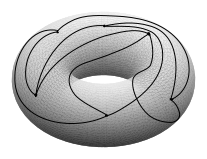
\includegraphics[scale=1.5]{\figdir/k-3-3-on-torus.pdf}
      \caption{$K_{3,3}$ on a torus. Apologies for the strange color
        theme; due to the author's partial colorblindness, more
        standard palettes were hard to work with.} \qedhere
    \end{figure}
  \end{sproof}
\end{leftbar}


\subsection{Definitions}
We define (oriented) \emph{virtual knots} in terms of signed Gauss
codes.
\begin{definition}[Virtual Knot]
  A \emph{virtual knot} is a string $コ$ of $2n$ characters such
  that for each $k = 1, \ldots, n$, for some choice of $\epsilon_k \in
  \set{+, -}$, the symbols $k^{\epsilon_k}_u$, $k^{\epsilon_k}_o$
  each appear in $コ$ exactly once.
\end{definition}
Compare with \cref{def:signed-gauss-code}. Here, instead of defining
Gauss codes in terms of knots, we've defined knots in terms of Gauss
codes. Returning to our analogy with $\CC$ and $\RR$, this would be
like defining $\CC$ as ``the set of all roots of single-variable
polynomials with real coefficients.''\footnote{To see this, note that
  for any $z \in \CC$, $(x - z) \cdot (x - \ol{z})$ has real
  coefficients.}

We define equivalence for virtual knots as follows:
\begin{definition}[Equivalence of Virtual Knots]
  We say two virtual knots $K_1$, $K_2$ are \emph{equivalent} if $K_1$
  can be transformed into $K_2$ by a finite sequence of Gauss code
  Reidemeister moves (this time without the planarity constraints on
  Reidemeister II).
\end{definition}
How do we interpret virtual knots and their equivalence geometrically?
Treating this question in full would take us beyond the scope of our
purposes today, but we will give a high-level overview.\footnote{For
  more, the reader is encouraged to investigate \cite{Carter2002May}}
Our first order of business is to define virtual knot diagrams.
\begin{definition}[Virtual knot diagram]
  A \emph{virtual knot diagram} is defined identically to the
  classical case, only now we include special \emph{virtual}
  crossings that we insert whenever we're forced to violate planarity
  to connect strands together. Virtual crossings are denoted by
  circles, as in \cref{fig:virtual-crossing}.
\end{definition}
\begin{figure}[H]
  \centering
  \includegraphics[scale=1.5]{\figdir/virtual-crossing.pdf}
  \caption{A virtual crossing}
  \label{fig:virtual-crossing}
\end{figure}
\begin{note}
  Virtual crossings do not appear in the signed Gauss code. This is
  because there's a sense in which they're not really ``there'' ---
  rather, they're an artifact of our projection into $\RR^2$. We'll
  expand on this below.
\end{note}
\begin{example}
  Consider the virtual knot given by $1^+_o 2^+_o 1^+_u 2^+_u$. If we
  were to try and interpret this as a classical knot, we'd run into
  some problems:
  \begin{figure}[H]
    \centering
    \includegraphics[scale=1.5]{\figdir/virtual-knot-example-classical.pdf}
    \caption{Now what?}
  \end{figure}
  Note, there's no way to connect the strand to crossing $2$ in the
  desired manner without introducing a \emph{new} crossing along the
  $(2^+_o, 1^+_o)$ semiarc. Hence, we employ a virtual crossing, which
  allows us to complete the diagram without problems.
  \begin{figure}[H]
    \centering
    \includegraphics[scale=1.5]{\figdir/virtual-knot-example.pdf}
    \caption{Virtual diagram}
    \label{fig:virtual-trefoil-grid-diagram}
    \qedhere
  \end{figure}
\end{example}
How do we interpret the resulting ``knot'' as an embedding? A hint
comes from \hyperlink{question-2}{\textbf{Motivating Question 2}}. As
we saw there, it's still possible to draw $K_{3,3}$ without having
edges cross each other if we work on a torus. Recalling the connection
between signed Gauss codes and planar graphs that we established
through the \hyperlink{def:diagram-graph}{diagram graph}, it seems
reasonable to think of virtual knots as knots that we draw on
thickened surfaces.\footnote{We need $[-\varepsilon, \varepsilon]$ of
  wiggle room to let the strands pass over/under each other.} In this
context, we see that virtual crossings don't really represent
\emph{real} crossings of the strands in our knot. Rather, they're
artifacts of our $2$D representations.
\begin{figure}[H]
  \centering
  \includegraphics[scale=1.2]{\figdir/virtual-knot-on-torus.pdf}
  \caption{An example of how we might obtain something like
    \cref{fig:virtual-trefoil-grid-diagram}.}
  \label{fig:virtual-knot-on-torus}
\end{figure}
Some care has to be taken in reworking our interpretation of what it
means for knots to be ``equivalent'' in this new context --- e.g., it
seems we might be able to get two inequivalent unknots by drawing
closed loops longitudinally / latitudinally on the surface. We will
not worry too much about this today; we're only interested in the
combinatorial aspects. For more, the reader is encouraged to look at
\cite{Carter2002May}.

By carefully studying \cref{fig:virtual-knot-on-torus}, the reader
might realize that performing Reidemeister moves on the surface of the
torus can actually introduce extra virtual crossings into our $2$D
projection.\footnote{This can also be derived entirely from looking at
  the signed Gauss code Reidemeister moves without planarity
  constraints.} This suggests that the purely diagrammatic
Reidemeister moves are insufficient for manipulating virtual
diagrams.\footnote{Of course, by definition the signed Gauss code
  Reidemeister moves still suffice for virtual equivalence.} Indeed
this is the case. To work purely in terms of diagrams, it's necessary
to introduce an expanded moveset, which is given by adding the
following four operations:\footnote{Note that as with the Reidemeister
  moves, one should actually include all possible combinations of
  orientations / connectivities on the diagrams above.}
\begin{figure}[H]
  \centering
  \begin{subfigure}[t]{0.5\textwidth}
    \centering
    \includegraphics[scale=.575]{\figdir/virtual-r1.pdf}
    \caption{Virtual Reid.\ I}
    \label{fig:virtual-r1}
  \end{subfigure}%
  ~
  \begin{subfigure}[t]{0.5\textwidth}
    \centering
    \includegraphics[scale=.575]{\figdir/virtual-r2.pdf}
    \caption{Virtual Reid.\ II}
  \end{subfigure}\\[1.5em]
  \begin{subfigure}[t]{0.5\textwidth}
    \centering
    \includegraphics[scale=.5]{\figdir/virtual-r3.pdf}
    \caption{Virtual Reid.\ III}
    \label{fig:virtual-r1}
  \end{subfigure}%
  ~
  \begin{subfigure}[t]{0.5\textwidth}
    \centering
    \includegraphics[scale=.5]{\figdir/virtual-r4.pdf}
    \caption{Mixed Reid.\ III}
  \end{subfigure}
  \caption[The virtual moves]{The virtual moves. Note that in the
    cases of Virtual Reid.\ II and Virtual/Mixed Reid.\ III, we should
    really be displaying analogues for \emph{all} of the classical
    moves (i.e., the different possible combinations of
    connectivities/orientations)}
\end{figure}
Together with the 3 standard diagrammatic Reidemeister moves, these
are sufficient to fully encode equivalence of virtual knot diagrams.

\section{A Very Brief Note on Unknotting Moves}
It is very important to note that although they might look similar to
the other virtual diagram moves, the following are \emph{not} valid
local modifications for virtual knot diagrams.\footnote{Once more, one
  should really be considering all possible orientations /
  connectivities for these moves.}
\begin{figure}[H]
  \centering
  \begin{subfigure}[t]{0.5\textwidth}
    \centering
    \includegraphics[scale=.5]{\figdir/forbidden-move.pdf}
    \caption{Forbidden Move I}
  \end{subfigure}~
  \begin{subfigure}[t]{0.5\textwidth}
    \centering
    \includegraphics[scale=.5]{\figdir/forbidden-move-2.pdf}
    \caption{Forbidden Move II}
  \end{subfigure}
  \caption{The Forbidden Moves}
\end{figure}
In fact, if we were to allow this move together with the others, it
would be sufficient to unknot \emph{any} knot, virtual or classical!
See
\href{https://www1.cmc.edu/pages/faculty/VNelson/unknottingthetrefoil.html}{here}\footnote{In
  case the link doesn't work, the url is
  \url{https://www1.cmc.edu/pages/faculty/VNelson/unknottingthetrefoil.html}.}
for an excellent step-by-step demonstration of unknotting the trefoil
using these moves.

The forbidden moves are examples of \emph{unknotting move}. These are
typically defined in terms of modification rules for diagrams, but
we'll define them below in terms of Gauss codes, since we're trying to
move in more combinatorial directions.
\begin{definition}[Unknotting Moves \& Unknotting Sequence]
  An \emph{unknotting move} is a modification rule for the Gauss code
  such that, together with the Gauss code Reidemeister moves, the
  operation is sufficient to reduce any Gauss code to one for the
  unknot (e.g., the empty string).

  Such a sequence of Gauss codes + Reidemeister moves is called a
  \emph{unknotting sequence}.
\end{definition}
\begin{example}
  The forbidden moves displayed above act on the Gauss code by
  exchanges of the form
  \[
    (\ldots, i, \ldots, i, j, \ldots, j, \ldots)
    \mapsto
    (\ldots, i, \ldots, j, i, \ldots, j, \ldots)
    % (\ldots, i, j, \ldots, j, \ldots, i, \ldots) \mapsto (\ldots, j,
    % i, \ldots, j, \ldots, i, \ldots).
  \]
  together with the appropriate choices of $\set{u,o}$ and $\set{+,
    -}$ (note, the middle $j,i$ always have the same $u$/$o$ label).
  Adding in the versions with other connectivities and orientations
  gets us moves of the form
  \[
    (\ldots, j, \ldots, i, j, \ldots, i, \ldots) \mapsto (\ldots, j,
    \ldots, j, i, \ldots, i, \ldots),
  \]
  again with the corresponding choices of $\set{u,o}$ and $\set{+,-}$.
  Hence we see that these moves allow for essentially arbitrary
  permutations of the Gauss code.
\end{example}

One of the reasons unknotting moves are fascinating is because it
seems they could offer us a nice way to define explicit algebraic
structure on knots. For instance, consider the following: let $K$ be a
knot given by some Gauss code $コ_K$, and let $\sigma_1, \sigma_2,
\ldots, \sigma_n$ be an unknotting sequence for $コ_K$. If we use
$コ_\maru$ to denote the Gauss code for the unknot, we think of this
process as follows:
\[
  (\sigma_n \circ \sigma_{n-1} \circ \cdots \circ \sigma_{2} \circ
  \sigma_1) (コ_K) = コ_\maru.
\]
But then note, since the $\sigma_i$ all have well-defined notions of
``inverses,'' we can also write
\begin{align*}
  コ_K
  &= \pn{\sigma_n \circ \sigma_{n-1} \circ \cdots \circ \sigma_2 \circ
    \sigma_1}^{-1} (コ_K) \\
  &= \pn{\sigma_1^{-1} \circ \sigma_2^{-1} \circ \cdots \circ
    \sigma_{n-1}^{-1} \circ \sigma_n^{-1}}(コ_K).
\end{align*}
That is, we can express $K$ in terms of a ``recipe'' for building $コ_K$
from the unknot! This idea becomes even more tantalizing when we see
just how simple these moves can be:
\begin{proposition}\label{prop:classical-unknotting}
  Let $K$ be a \emph{classical} knot represented by a Gauss code $コ_K$.
  Then being allowed to exchange $k^{\epsilon_k}_u$,
  $k^{\epsilon_k}_o$ arbitrarily yields an unknotting move.
\end{proposition}
\begin{sproof}[Sketch]
  Note, this corresponds to switching which strand is on top vs.\ on
  bottom at any given crossing. Using this, one can switch the
  crossings until $コ_K$ represents a knot that is always passing
  ``underneath'' itself.\footnote{In terms of the Gauss code: If one
    considers the sub-string consisting of the first time we encounter
    each crossing $k$, all of them would be labeled with
    overcrossings.} A simple pigeonhole principle argument can be
  applied to show that there must always exist a simplifying
  Reidemeister I or Reidemeister II move in this situation.
\end{sproof}
\begin{remark}
  Using this, one can show that the move defined by ``flipping $k$
  consecutive crossings'' is an unknotting move as well. The idea is
  that we can derive the single-crossing flip by simply inserting
  $k-1$ Reidemeister I loops into $コ_K$ after some crossing, flipping
  all $k$ of these, and then removing the $k-1$ Reidemeister I loops.
  Note too that the single-crossing-flip can be used to derive the
  $k$-crossing version. In this sense, the two are ``equivalent.'' For
  more on these ideas, see \cite{Nakanishi1994Jun}.
\end{remark}
One might note that the unknotting moves we've discussed so far appear
to have a very ``symmetric group'' flavor to them. Indeed, both of our
examples seem to be encoding transpositions of some flavor, which we
might recall are the generators for $S_n$. We spend the next chapter
describing one way of making this explicit. Before that, we have a
brief discussion of how \emph{if} we were able to make this unknotting
move representation algebraically well-defined in an
efficiently-computable way, then we would be able to reduce knot
equivalence to the unknot detection problem.

\subsection{Addendum: Reducing Knot Equivalence to the Unknotting
  Problem}
Currently, we do not have an NP solution for determining knot
equivalence (\cite{Lackenby2016Apr}). However, we do have an NP
solution for determining if a given knot is unknotted
(\cite{Lackenby2013Feb}). \emph{If} something like the following were
true, then we would be able to explicitly construct a reduction
showing knot equivalence is NP. We should be very clear that we expect
\cref{prob:unknotting-transformation} is almost certainly impossible,
but we have no proof of this. We remain hopeful that a related
approach could prove fruitful (or at the very least, interesting),
which is why we have chosen not to omit its mention.
\begin{problem}\label{prob:unknotting-transformation}
  Let $K_0, K_1$ be tame knots represented by Gauss codes $コ_{K_0}$,
  $コ_{K_1}$. Given an unknotting sequence $\Sigma_{K_0}$ for $K_0$,
  does there exist a polynomial-time algorithm for converting
  $\Sigma_{K_0}$ to $\Sigma_{K_1}$, such that $\Sigma_{K_1}$ unknots
  $K_1$ iff $K_0 \cong K_1$?
\end{problem}
We actually need a second proposition as well, but it is
straightforward in the case of classical knots. We have not considered
the virtual case, but we imagine an analogous version holds.
\begin{proposition}
  Given an $n$-crossing classical knot $K$ represented by a Gauss code
  $コ_K$, there exists an $O(n)$ time algorithm for computing an
  unknotting sequence reducing $コ_K$ to a (non-simplified) Gauss code
  for the unknot.
\end{proposition}
\begin{sproof}
  One can simply traverse $コ_K$, checking at each crossing
  $k_{x_k}^{\epsilon_k}$ whether we have encountered $k$ in the Gauss
  code already or not. If we haven't, then we apply a crossing-flip
  move if needed to ensure $x_k = o$. Else, we continue. Per the
  argument in \cref{prop:classical-unknotting}, the resulting Gauss
  code represents an unknot.
\end{sproof}
This gives us the following.
\begin{proposition}
  If \cref{prob:unknotting-transformation} is true, then the
  (classical) knot equivalence problem is polynomial-time reducible to
  the unknotting problem, and hence NP.
\end{proposition}
\begin{sproof}[Sketch]
  Given $K_0$, compute $\Sigma_{K_0}$. Apply
  \cref{prob:unknotting-transformation} to yield $\Sigma_{K_1}$. Apply
  $\Sigma_{K_1}$ to $K_1$. Then the result is an unknot iff $K_0 \cong
  K_1$, hence we have a polynomial-time reduction to unknot detection.
\end{sproof}
As we've said, \cref{prob:unknotting-transformation} seems like far
too much to hope for. However, other approaches can yield similar
reductions, and we wonder whether there's one that could yield a
feasible approach to demonstrating knot equivalence is NP. For now,
however, this seems out of reach.

We'll now switch our focus to examining an algebraic formalism for
knots that encodes the idea of ``unknotting moves \emph{generating}
knots, together with Reidemeister equivalence.'' This is the focus of
\cref{chap:connections-to-sn}.
% \begin{problem}
%   Given $K_0$, $K_1$, does there exist a polynomial-time algorithm for
%   converting the diagrams of $K_0$, $K_1$
% \end{problem}



% One might get the feeling that there are connections with the
% Symmetric group lurking here.



% 1 2 3 -1 -2 -3

% {\color{blue} }

% \subsubsection{Unknotting moves and \#}
% As we discussed in the introduction section, we want to create
% algebraic structures to better understand how to build knots. The two
% most popular such operations are \emph{unknotting moves}, which let us
% reduce any knot diagram to the \emph{unknot}; and the \emph{connected
%   sum} (denoted $\#$), which sort of acts like a ``multiplication''
% operation on knots.

% \begin{definition}[Unknotting move]
%   An \emph{unknotting move} $u$ is a local modification of a diagram
%   such that $u$ together with the Reidemeister moves is sufficient to
%   reduce any knot diagram to the unknot.
% \end{definition}
% There are many families of unknotting moves, but the simplest one is
% a \emph{crossing exchange}. Essentially, given some crossing in a
% knot, we just flip which strand is on top. In terms of the signed Gauss code,
% this is a move like
% \[
%   (\cdots, i_{x}^{\epsilon}, \cdots, i_{y}^\epsilon, \cdots)
%   \mapsto
%   (\cdots, i_{y}^{\epsilon}, \cdots, i_{x}^\epsilon, \cdots)
% \]
% Note, it follows that by playing the unknotting sequence in reverse,
% we can also use unknotting moves to \emph{construct} arbitrary knots
% starting from the unknot! We'll be studying this a lot next semester.%  (this is the motivating idea behind our
% % project).


% As it turns out, in order to understand the properties of these
% objects, it is most natural to first try and define them for wild
% knots, then turn tame knots \emph{into} wild knots in a controlled
% manner. In the next chapter, we examine one way of doing this
% conversion from tame knots to wild knots.



%%% Local Variables:
%%% TeX-master: "../../kobayashi-thesis"
%%% End:
